
\chapter{Referencial Teórico}

% Começando do básico do básico do básico

Computadores são sistemas incrivelmente complexos. Inúmeros componentes com
papeis específicos necessitam de se intercomunicar para executar a mais simples das
tarefas. Dessa forma, para compreender seu funcionamento, se faz o uso de
camadas de abstrações.

% Camadas de abstrações
Essas camadas exercem funções diferentes e são visíveis de acordo com seu uso
--- um usuário final não precisa saber programar para usar um processador de
texto; da mesma forma, um programador não necessita saber da estrutura dos
circuitos internos. Cada camada possui seu domínio, sendo as mais próximas do
usuário final denominadas de ``alto-nível'' e as mais próximas dos transistores
e fios, ``baixo-nível''. Observe a figura \ref{camadas}, especificada de acordo
com Murdocca \cite{principles}.

% As várias camadas bonitinhas
\begin{figure}[ptb]
  \begin{center}
    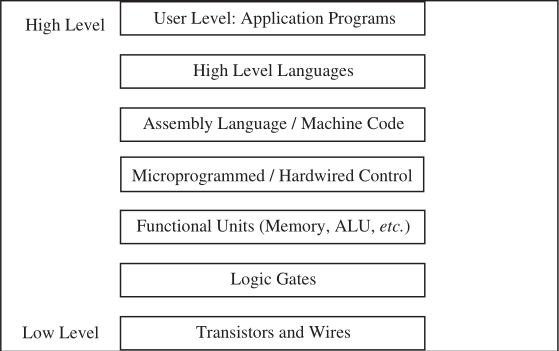
\includegraphics[scale=.6]{imagens/1_camadas}
  \end{center}
  \caption{Camadas de abstração de um computador.}
  \label{camadas}
\end{figure}

Iremos definir conceitos básicos, utilizados ao longo do trabalho. Nossa abordagem
será \textit{top-down}, significando que os conceitos serão explicados do nível
mais abstrato até o mais concreto nível de \textit{hardware}.

\section{Arquitetura de Processadores}

CPU

\section{Controladores de Dispositivos Externos}

CPU

\section{Sistemas Operacionais}
% kure

CPU

\section{Carregadores}
% kure

CPU

\section{Ligadores}

%Após arquivos objeto de um ou vários módulos de compilação serem gerados por um montador, é preciso combiná-los em um único arquivo que pode ser carregado para a memória por um programa carregador do sistema operacional.


\section{Montadores}

Montadores são programas que traduzem um módulo de compilação em linguagem \textit{assembly} para uma versão em linguagem de máquina. O armazenamento desta versão é feito em um arquivo objeto. Como veremos em uma seção adiante, um arquivo objeto é uma versão binária de um módulo de compilação, que geralmente fica a um passo de poder ser carregada para execução.

\subsection{Linguagem de máquina}

Anteriormente vimos que uma linguagem de montagem, ou linguagem \textit{assembly}, é formada por símbolos mnemônicos, ou palavras-chave, que identificam as instruções que um processador é capaz de executar.

A etapa seguinte à compilação é a montagem. Nesta etapa, é necessário traduzir os mnemônicos \textit{assembly} para sequências de \textit{bits}. Um \textit{bit} é um dígito que pode assumir apenas o valor 0 (zero) ou o valor 1 (um). Durante a execução de um programa, estas sequências de \textit{bits} serão diretamente interpretadas por uma \textit{CPU}.

Costuma-se dizer que a etapa de montagem é onde está localizada a interface \textit{software}-\textit{hardware}. Uma \textit{ISA} - \textit{Instruction Set Architecture}, ou Arquitetura de Conjunto de Instruções - é uma especificação das instruções que uma implementação de processador digital deve fornecer. Esta especificação estabelece os formatos que as sequências de \textit{bits} geradas por montadores devem seguir.

\subsection{Algoritmos de montagem}

AE

% kure
\section{Compiladores}

% Importância de Compiladores
No âmbito da computação em geral, compiladores são uma das mais importantes
aplicações.  É impossível imaginar um sistema computacional sem alguma forma de
compilação. Compiladores estão presentes em quase todas as camadas de abstração
de um computador.

% Calma aê, vamos começar lá de cima
Porém, para compreender o conceito de compilador é necessário estudar sobre
linguagens de programação e o processo de tradução.

\subsection{Linguagens}

% Linguagem é muito abstrato
% CITAR COISA ABSTRATA SOBRE LINGUAGENS
\textit{Linguagem} é um conceito abrangente. Enquanto que diferentes áreas do
conhecimento definam \textit{linguagem} por formas específicas, para nosso
trabalho será suficiente uma definição geral.

% OK, lá vai... Linguagem
Linguagem é um sistema de comunicação - um conjunto de regras e convenções que
permitem a interação entre dois pares. Dialetos humanos (português, inglês,
francês...) são exemplos de tais sistemas de comunicação. Cada um destes define
acordos (gramáticas, sintaxe, morfologia) que permitem a troca de mensagens
entre pessoas de mesmo grupo.

% Coisas interessantes sobre linguagem
Dessa forma, pares que queiram interagir entre si necessitarão de trocar
conhecimento através de mensagens na mesma linguagem. Caso haja comunicação por
duas linguagens diferentes, ocorrerão erros de compreensão, desentendimentos e
até completa inabilidade de se comunicar.

\subsection{Linguagens de Programação}

% Linguagem de programação
Partindo para o domínio computacional, há o conceito de linguagens de
programação. Estas possuem objetivo de comunicar instruções de seres humanos
para máquinas. Mais especificamente, possuem o objetivo de determinar o que
computadores devem fazer - como estes são programados a agir.

% Programação -> Máquina
Linguagens de programação são destinadas a expressar idéias concebidas por seres
humanos. Dessa forma, precisam se aproximar da linguagem natural - forma de
comunicação natural entre seres humanos.  Devido à construção física de
máquinas, computadores precisam de instruções em formato bastante diferente do
oferecido pela linguagem natural - quanto mais de linguagens de programação.

\subsection{Linguagem de Máquina}

% Linguagem de máquina
É nesse conceito que se define a linguagem de máquina, também conhecida como
código de máquina. São conjuntos de instruções (ou ordens) que determinam como a
máquina irá se comportar. Controla-se um computador ao agrupar várias dessas
instruções em ordens específicas.

% Não é linguagem de programação
Linguagem de máquina se diferencia das linguagens de programação no sentido de
que não são facilmente compreendidas por seres humanos. Enquanto que linguagens
de programação se aproximam da linguagem natural, linguagem de máquina é
definida pela construção física dos componentes de cada máquina.

\subsection{Linguagens de Alto e Baixo nível}

% Linguagens de alto-nível e baixo-nível, exemplos

Com linguagens em pontos tão extremos, como alto e baixo nível, se torna
impossível a comunicação entre pares que as utilizem. Necessita-se de um meio
de conversão entre estas.

\subsection{Tradução}


% Tradução - duas linguagens
% CITAR COISA ABSTRATA SOBRE LINGUAGENS

% Exemplos de tradução

\subsection{Compiladores}

% Finalmente, compiladores
% CITAR CONCEITO DE COMPILADORES
Compiladores são programas que transformam código-fonte escrito em uma linguagem
de programação em outra. Eles fazem o processo de tradução, em geral de
linguagens de alto nível para linguagens de baixo-nível.

\section{Criptografia}
% kure

CPU

